% !TEX root = ../thesis.tex

% Tutkimustuloksien merkitystä on aina syytä arvioida ja tarkastella
% kriittisesti. Tässä osassa on syytä myäs arvioida tutkimustulosten luotettavuutta.

% At this point, you will have some insightful thoughts on your implementation
% and you may have ideas on what could be done in the future. This chapter
% is a good place to discuss your thesis as a whole and to show your professor
% that you have really understood some non-trivial aspects of the methods you
% used. . .

\documentclass[thesis.tex]{subfiles}

\begin{document}

\chapter{Discussion}
\label{chapter:discussion}

This chapter discusses the design decisions taken during the implementation of the application and the findings made based on the the raw result data and the parts of it summarized in \ref{chapter:results}. Last, challenges faced during the project and an outline for future research work are presented. Motivation behind some of the design choices mentioned earlier in the writing are not reiterated here, and the interested reader is instead advised to refer to Chapter \ref{chapter:design-implementation} and the related appendices \ref{appendix:camera-module} and \ref{appendix:capture-presets}.

\section{Design Choices}

One of the challenges early on in the project was the capture of a taggant's photoexcitation. A 3D printed version of the camera module had been developed prior the project for demonstration purposes. It provided good isolation from ambient light and even a built-in slot for different diffraction gratings. It however did not include an integrated light source, and taggants were instead excited manually by toggling a UV flashlight (Nightsearcher UV 365). A programmatic control over the light source was required for product authentication purposes. And, as integration of a smartphone and a light source with the existing 3D printed mold proved difficult, a cardboard prototype was implemented, as presented in \ref{chapter:camera-module}.

The smartphone torch light in both the Samsung S4 and Lumia 1020 did not emit the right kind (wavelength) of light to be able to excite the taggants, and thus, an external light source was required. An external light source would also help in normalizing differences between smartphones and the various kinds of wavelengths their torch lights emit. Programmatic control of the light source required a connection to be established between the smartphone and the light source. Cross-modal communication by means of light signals proved to be a straightforward solution. Connecting the two devices via WiFi, Bluetooth or cable would have added unnecessary complexity in terms of the use case.

As one of the goals of the project was to be able to compare results across different smartphones (as per \ref{R1}), the capture parameters needed to be standardized. For this purpose a set capture presets were defined (see Table \ref{table:capture-presets}). The preset values for the \emph{interval} duration were configured based on the taggants. As described in \cite{luminova}, the Luminova\textregistered pigments have a fairly long emission duration. For a smartphone to be able to capture any significant change in the emission the interval also needed to be long. The appropriate intervals of 200, 400 and 600ms were eventually derived empirically. The preset resolutions were set to the highest preview frame resolution supported by the given platform. As Windows Phone 8.1 did not support preview resolutions higher than $1280\times720$px only three presets were defined for the Lumia 1020.

Different focus strategies were applied depending on the platform. Android 4.4.2 does not support setting focus to a fixed minimum distance. Therefore, macro focus mode was used to guarantee the Samsung S4 could still acquire accurate focus around its MFD. The macro focus mode however required the use of the focus light. The torch light was therefore not used on the Samsung S4 to avoid triggering the light source twice -- the focus light would function as the trigger instead. On the Lumia 1020 the focus could be set to a fixed minimum distance (MFD), and the (torch) light was used only as the light source trigger.

A number of parameters were set to a fixed value (see Table \ref{table:capture-presets-fixed}). The number of frames (samples) to capture per fingerprint was fixed at five frames. It was empirically observed that additional frames would not provide much data due to decreasing Signal-to-noise ratio (SNR). Furthermore, capturing more frames would have led to worse experience for the user as the capture and processing times would have gotten longer. Capturing three or four frames could have provided similar results, but as emission peaks could still be detected even after 3000ms for some of the taggants, the frame count was not adjusted. Moreover, it would be trivial to retroactively compute results against four or less frames if necessary.

The camera white balance was set to the \emph{Daylight} preset value as Android 4.4.2 does not support manual white balance adjustment. The Daylight preset was chosen over other available white balance presets as it typically applies the least compensation and corresponded well with the color temperature (5600K) of the experiment light source (Yongnuo YN565EX). The Daylight preset represents roughly a temperature of 5500-6500K depending on the vendor.

Other capture parameters set to a fixed value were \emph{delay} and \emph{ISO}. The time to delay the capture of the first frame (after the light source has been triggered) was determined empirically by observing when the focus light of the Samsung S4 would no longer introduce artefacts. An example of the artefact caused by the interference from the S4's focus light is presented Figure \ref{figure:artefacts}. The interference was believed to have been caused by the decay of the smartphone's led light interfering with the preview feed signal. The Lumia 1020 exhibited no such behaviour. The capture ISO was set to \emph{auto} as Samsung S4 was unable to lock exposure for the time of the capture when a manual ISO value was used. This was believed to be a bug in the camera API of Android 4.4.2 when frames are captured from the preview feed. Ideally, a low ISO value of ISO100 would have been used to avoid introducing any unwanted noise to the pipeline.

The motivation for using hue and hue-saturation histogram analysis as the basis of the fingerprint matching was largely inspired by how luminophores are studied in chemistry by means of spectroscopy. The idea of the histograms was to provide a rough estimate of the ``emission spectrum'' (color distribution) of the taggant. The capture of a proper emission spectrum would have required a way to diffract the incident light (e.g. via a diffraction grating) and apply proper color calibration for translating RGB values into wavelengths. The parameter values used for the fingerprint and histogram methods to analyze and match the capture data were largely based on apriori assumptions and observations how the results changed when a given parameter was adjusted.

Binary thresholding was used as the primary filter due to its simplicity and fit for the context. As the frames consisted of small color blobs on a dark background the dark pixels on the background were easily singled out by a binary thresholding level of 15\%. The hue bin size was set to 180, which is also the maximum number of hue bins OpenCV supports (for 8-bit images). Internally OpenCV's \emph{calcHist()} function encodes the hue values from 360 down to 180 for better performance. A bin count of 60 was used for saturation as it was assumed that smaller saturation bin sizes would increase computation time and have only a low impact on the final score. The persistance threshold used by the fingerprint method for peak selection was set to 20\% purely based on what threshold would provide neither too many nor too few peaks in general. The implications of this are briefly discussed in Chapter \ref{chapter:findings}. The penalty weight, damping coefficient and delta threshold of the fingerprint method were also derived empirically by first assigning them logical initial values and adjusting those until the results of randomly selected samples of the data improved.

While the tracing process is storage backend agnostic, a NoSQL database solution was selected over a relative DBMS technology due to the better schema flexibility of NoSQL databases. Furthermore, a document-based NoSQL DBMS is ideal for storing JSON data like for example fingerprint documents (Appendix \ref{appendix:fingerprint}). A flexible schema also allows changing document fields without costly migrations, which speeds up the development cycle (imperative for new projects) and helps in including various kinds of metadata to documents (e.g. vendor specific fields). CouchDB was chosen as the underlying NoSQL implementation for its wide adoptance and support for client-side data replication (through PouchDB).

\section{Findings}
\label{chapter:findings}

Based on Figure \ref{figure:taggants} it is apparent that the shape and size of sibling fingerprints vary. This due to the fact that luminophore was pipeted on the cartons by hand in an uncontrolled environment. Another side effect of the manual taggant creation process can be seen in the non-uniform luminophore concentration of taggant \emph{13SVb} -- the highly concentrated areas of the taggant have gotten overexposed. The relative size difference between the taggants captured with the Samsung S4 and Lumia 1020 is due to the difference in the lens MFD (10cm and 15cm, respectively). Moreover, taggant \emph{S} is hardly visible (its visibility in the figure has been improved for demonstration purposes). This could be due to the light source not emitting the appropriate wavelength to excite the taggant or the sensor's low sensitivity to the blue pigment (\emph{DB} in Appendix \ref{appendix:taggants}). Differences in the visibility of the taggant between the Samsung S4 and Lumia 1020 indicates the latter. The poor sensibility of the blue pigment is also seen in the close similarity of the \emph{13SP} and \emph{P} taggants. Based on these discrepancies alone it is obvious that taggants captured by the Samsung S4 and Lumia 1020 can not be unambiguously compared with another.

The fingerprint clusters visualized in Figure \ref{figure:clusters} suggest that histogram method outperforms the fingerprint method. It is able to find 50\% more clusters in the corpus as well as cover over 95\% (137/144) of all the fingerprints (vs. 66,67\% of the fingerprint method). Furthermore, the clusters are of better ``quality'' as there are several groups of 2-4 sibling fingerprints -- clusters that have similar size and color. Based on the results of the clustering taggants \emph{24VP} and \emph{24SP} perform the best while \emph{13SV} and \emph{24SV} provide mixed results.

Figure \ref{figure:tags_presets} provides more insight into the performance of individual taggants and presets. Unsurprisingly, long intervals help distinguish the taggants, although no significant change in the performance between presets of 200ms and 400ms interval can be observed. The Windows Phone presets (\emph{wp}) fare better, which is expected due to the higher quality camera in the Lumia 1020. The relatively poor performance of taggant \emph{13SV} can be explained by the overexposure artefact in its \emph{b} sample and the fact that it noticeably differs from its sibling sample as depicted in Figure \ref{figure:13SV}. In the case of taggant \emph{S} on the other hand, the drop in the number of matches can be attributed to the poor detectability of the blue pigment causing low SNR. Somewhat surprising is how relatively few times taggant \emph{13SP} is matched by the histogram method in comparison to taggant \emph{P}. The raw result data shows that a good number of \emph{13SP} taggants actually match closer to taggant \emph{P} than their siblings. The pipeline is unable to efficiently differentiate the similarity of taggants \emph{13SP} and \emph{P}.

\begin{figure}[h!]
  \centering 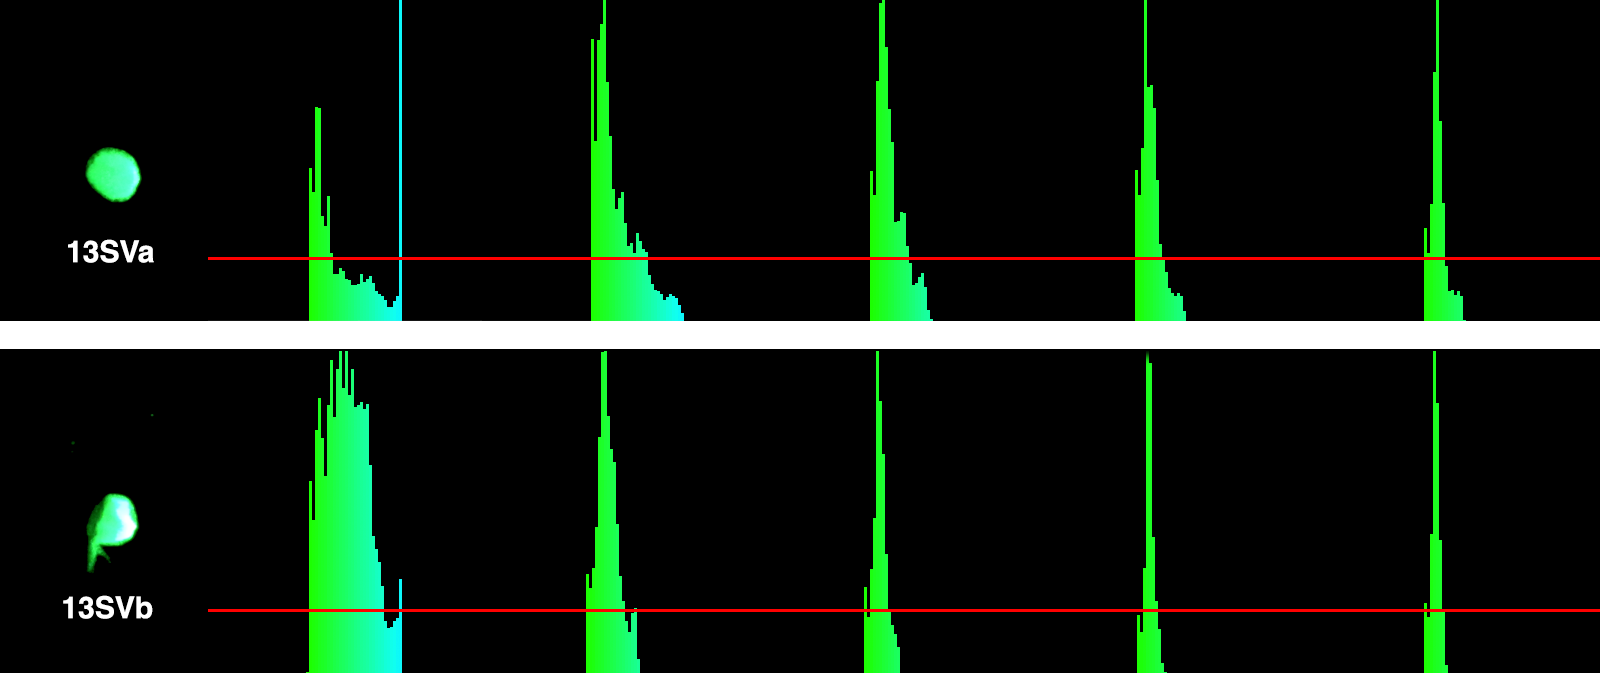
\includegraphics[page=1,width=\textwidth]{images/findings/13SV}
  \caption{Due to an artefact introduced during the taggant preparation the first two samples of taggant \emph{13SVb} were largely dissimiliar compared to its sibling \emph{13SVa}. The red horizontal line depicts the persistance threshold.}
  \label{figure:13SV}
\end{figure}

Based on Figure \ref{figure:tags_presets} increasing $B_{count}$ from three to six fingerprints seems to have minimal effect on the number of matches found. The success rate and precision curves given in Figures \ref{figure:match_precision_fingerprint} and \ref{figure:match_precision_histogram} support this observation: after a certain level of $B_{margin}$ the success rate stagnates regardless of the $B_{count}$, while precision continues to decrease. Moreover, a combination of a high $B_{count}$ and $B_{margin}$ degrades user experience as a larger number of matches (products) would be retrived for the user to choose from. An ideal combination of $B_{margin}$ and $B_{count}$ seem to range from 50-80\% and 3-6 for the fingerprint method, and from 20-40\% and 3-8 for the histogram method. If anything, excessively increasing $B_{margin}$ will only lead to more false positives for the user to filter. On the other hand, as seen in Table \ref{table:match_precision_count1}, if only the best match ($B_{count} = 1$) was processed, the user would be displayed the correct product in less than 50\% of the time.

As indicated by the clustering in Figure \ref{figure:clusters} and the match distributions in Figure \ref{figure:tags_presets} taggants \emph{24VP} and \emph{24SP} provide good results, especially with presets of the 600ms interval. Higher pigment concentrations seem to improve the SNR. When the boundary conditions are set to $B_{count} = 4$ and $B_{margin} = 30\%$ the success rate and precision of \emph{24SP} is 100\% and 84,26\%, and respectively 94,44\% and 57,35\% for \emph{24VP} using the histogram method. Given this it is surprising that the performance of \emph{24SV} is significantly worse (success rate: 55\%, precision: 46\%). The raw data shows that \emph{24SV} comes very close to matching its siblings. In 16 out of the 18 tracings (9 presets $\times$ 2 samples) 50-100\% of the matches included the correct taggant (\emph{24SV}). Thus, the low the success rate of \emph{24SV} was largely due to the given method's inability to distinguish between presets.

Both of the methods were indeed better at distinguishing the fingerprints by the taggant rather than the preset as shown in Table \ref{table:match_precision_count1}. In the case of \emph{24SV} the $50\mu l$ addition of the green and blue pigments (\emph{G} and \emph{DB}) was not enough to produce any significant change in the emission as illustrated by Figure \ref{figure:SV} -- pigment \emph{DB} relaxes too \emph{slowly} for the sensor to capture any change.

\begin{figure}[h!]
  \centering 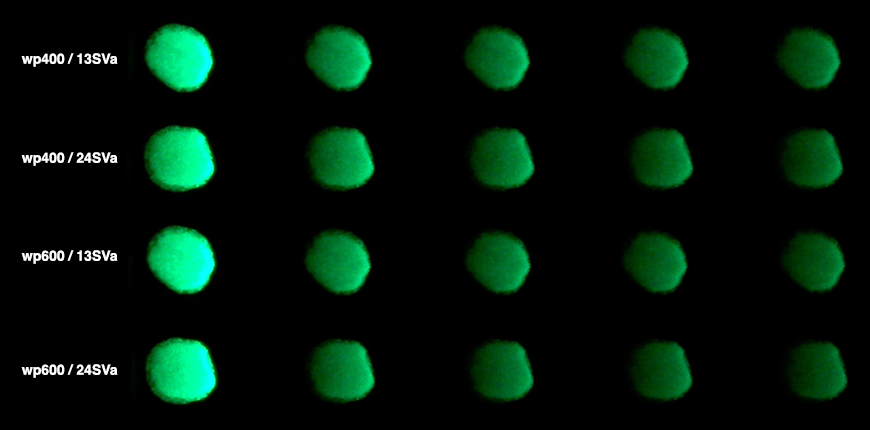
\includegraphics[page=1,width=\textwidth]{images/findings/SV}
  \caption{Regardless of the increase in luminophore concentration and capture interval duration from 400ms to 600ms no significant changes could be observed between taggants \emph{13SV} and \emph{24SV}.}
  \label{figure:SV}
\end{figure}

max success rate indicated by clustering
fingerprint method: more misses (histogram method more stable)
- margin std. deviation shows randomess/unstable feat

10. Anomalies \& Artefacts
  - wp\_600/13VPb: matches everything with fingerprint method, only a few with histogram
  - it was observed from the raw data that wp\_600/13VPb matched surprisingly poorly with rest of the corpus. This was due to (persistance threshold, residue afterglow?):
    % /Users/Make/Documents/dippa/app/luminotrace-native/corpus/data/wp_600/13VPb/2015-05-06-004852
    vs.
    % /Users/Make/Documents/dippa/app/luminotrace-native/corpus/data/wp_400/13VPb/2015-05-05-184418
  - bin count? less frames because such low SNR...

11b. How would the fingerprint method perform if...
  - bin count < 180
  - frames: 3/4



summary of the findings:

- histogram outperforms fingerprint method
- lumia outperforms s4
- long intervals provide better results
- taggant preparation process has a great impact
- fewer frames could suffice(?)
























\section{Challenges and Future Work}

Address RQs

\begin{comment}
Ideally, the taggants would have been captured through a diffraction grating (or a prism). Translate to wavelengths through proper color calibration.

There are mainly two modules responsible for the color-rendering accuracy of a digital camera: the former is the illuminant estimation and correction module, and the latter is the color matrix transformation aimed to adapt the color response of the sensor to a standard color space. These two modules together form what may be called the color correction pipeline.

RGB is a device-dependent color model: different devices detect or reproduce a given RGB value differently, since the color elements (such as phosphors or dyes) and their response to the individual R, G, and B levels vary from manufacturer to manufacturer, or even in the same device over time. Thus an RGB value does not define the same color across devices without some kind of color management.
\url{http://www.cis.rit.edu/~jxj1770/publications/paperEI_Xerox.pdf}
\url{http://www.cs.unc.edu/techreports/04-012.pdf}

% https://www.cs.unc.edu/~welch/media/pdf/Ilie2005_Calib.pdf
% Unfortunately most cameras—even of the same typedo not exhibit consistent responses. Figure 1 illustrates the
% differences between the responses of 8 cameras to the 24 colors of the GretagMacbeth [5] ColorCheckerTM chart
% imaged under the same illumination conditions and using the same hardware settings. The data shows that color
% values are significantly different from camera to camera. This is due for example to aperture variations, fabrication
% variations, electrical noise, and interpolation artifacts arising from the reconstruction of a full-resolution color image
% from a half-resolution Bayer pattern image

\end{comment}

- Equation \ref{equation:similarity-metric-no-peaks}: shortcoming of the fingerprint method?
  - analysis/match params are very static
- thus it be better to add some structural \& spatial similarity semantics (- more novel selection criterion) - analogies to existing solutions (InkSure \& CryptoGlyph)
  - alternative approach: colored dots form a discrete pattern, no grating necessary
- high res images could be used as camera APIs improve
% - The preview feed was used since the Android and Windows Phone versions (Kitkat and 8.1, respectively) lacked the proper support for burst mode (image capture at a predefined interval). Furthermore, frames could not be captured individually as Thus, there was no way to schedule the capture to take place at a specific interval.

- compensate for differences in the MFD by adjusting the zoom level (only if lossless zoom is available)
- YCbCr suffers from clipping (https://en.wikipedia.org/wiki/YCbCr)
- color calibration (requires use of RAW data)
  - CCD > CMOS koska parempi herkkyys
- device detection (automatic configuration, database per phone model)
- iOS support (ios with c++? On iOS this extra bridge is unnecessary as C++ code can directly invoke Objective-C APIs.)
- more efficient matching if done server-side (leverage histogram data directly?)
  - easy to switch over because the offline-first approach taken
- change management / how to handle updates \& different devices?
- use histogram method. Fingerprint method useful for querying/filtering?
- more sophisticated peak finding / matching algorithms
- use of diffraction grating and spectral analysis
- get hold of the device or man-in-the-middle (metadata works as a layer of indirection)
using a predefined username and password (easily extendable to a real user auth)
- CouchDB uses a traditional cookie based authentication scheme, and as such, applications can be vulnerable to CSRF attacks. However, the application has no CSRF attacks vectors as it the DBMS and the application server is read-only
Traditional Cookie-Based Auth (could be extended to Modern Token-Based Auth such as JWT)

% \subsection{Taggant}
- phosphorescence vs. fluorescence (infeasible coz time)
- Afterglow brightness is also proportional to the intensity of UV contained in the excitation light.
- LumiNova pigments originally developed for use in watch dials
- Erilaisilla hiloilla, suodattimilla, raoilla ja peileilla on ehdottoman tarkea tehtavansa riittavan resoluution aikaansaamiseksi ja jotta saadaan valituksi tarkka viritysaallonpituus ja saadaan minimoiduksi sironta ja taustaluminesenssi. aikaerotteisen maarityksen etuna on se, etta viritysvalo ehtii sammua kokonaan ja sirontailmioiden aiheuttaman taustan vaikutus poistuu. Pitka elinika mahdollistaa myos edullisen ja varsin yksinkertaisen laitteiston kayton.122,124
- idempotence of the luminphores (photobleach)


\end{document}